% =====================================================================
\partieENO{Le matériel}

Avant d'entrer dans les études, il faut savoir de quoi je dispose et combien tout cela coûte. Cette partie fait l'inventaire du matériel. J'explique d'abord comment je calcule les prix, parce que les vendeurs ne comptent pas tous dans la même monnaie. Je donne ensuite un seul grand tableau : ce que j'ai déjà en main et ce qu'il reste à commander, avec une photo, un prix en francs Pacifique (XPF) et un total.

\subsection{Comment les prix sont calculés}

Les prix d'Adafruit et de DFRobot sont en dollars américains, ceux des vendeurs français en euros. Pour tout mettre en francs Pacifique, je cherche d'abord combien de francs valent un dollar. J'en déduis ensuite le prix d'un article, en dollars puis en euros, et enfin les totaux.

\naturecalc{calcul de coût, à partir de prix relevés et d'hypothèses ; ce n'est pas une mesure}
\begin{demonstration}[taux de conversion du dollar en franc Pacifique]
\resultat{t = \dfrac{\qty{119,332}{XPF/EUR}}{\qty{1,1236}{USD/EUR}} \approx \qty{106,2}{XPF/USD}}
Je note $t$ le nombre de francs Pacifique que vaut un dollar, en XPF par USD. Je pars de deux égalités : un euro vaut \qty{119,332}{XPF}, et un euro vaut \qty{1,1236}{USD}. Les deux membres valent un euro, donc ils sont égaux :
\begin{align*}
\qty{1,1236}{USD} &= \qty{119,332}{XPF}
\end{align*}
Je divise les deux membres par \num{1,1236} pour isoler un seul dollar :
\begin{align*}
\qty{1}{USD} &= \frac{\qty{119,332}{XPF}}{\num{1,1236}}\\
t &= \frac{\qty{119,332}{XPF}}{\num{1,1236}\ \unit{USD}}\\
t &\approx \qty{106,2}{XPF/USD}
\end{align*}
J'arrondis à un chiffre après la virgule.
\end{demonstration}

\naturecalc{calcul de coût, à partir de prix relevés et d'hypothèses ; ce n'est pas une mesure}
\begin{demonstration}[prix d'un article vendu en dollars]
\resultat{P_{\text{XPF}} = P_{\text{USD}} \times t}
Je note $P_{\text{USD}}$ le prix de l'article en dollars, en USD, et $P_{\text{XPF}}$ son prix en francs Pacifique, en XPF. Un dollar vaut $t$ francs, donc $P_{\text{USD}}$ dollars valent $P_{\text{USD}}$ fois $t$ francs. Pour le régulateur de charge MPPT\ix{19} à \qty{120}{USD} :
\begin{align*}
P_{\text{XPF}} &= \qty{120}{USD} \times \qty{106,205}{XPF/USD}\\
P_{\text{XPF}} &\approx \qty{12744,6}{XPF}\\
P_{\text{XPF}} &\approx \qty{12740}{XPF}
\end{align*}
J'arrondis aux dix francs les plus proches.
\end{demonstration}

\naturecalc{calcul de coût, à partir de prix relevés et d'hypothèses ; ce n'est pas une mesure}
\begin{demonstration}[prix d'un article vendu en euros]
\resultat{P_{\text{XPF}} = P_{\text{EUR}} \times \qty{119,332}{XPF/EUR}}
Je note $P_{\text{EUR}}$ le prix de l'article en euros, en EUR. Un euro vaut \qty{119,332}{XPF}, donc $P_{\text{EUR}}$ euros valent $P_{\text{EUR}}$ fois \qty{119,332}{XPF}. Pour la batterie Yuasa à \qty{61,32}{EUR} :
\begin{align*}
P_{\text{XPF}} &= \qty{61,32}{EUR} \times \qty{119,332}{XPF/EUR}\\
P_{\text{XPF}} &\approx \qty{7317,4}{XPF}\\
P_{\text{XPF}} &\approx \qty{7320}{XPF}
\end{align*}
J'arrondis aux dix francs les plus proches.
\end{demonstration}

\naturecalc{calcul de coût, à partir de prix relevés et d'hypothèses ; ce n'est pas une mesure}
\begin{demonstration}[totaux du tableau]
\resultat{S = \qty{84873}{XPF}}
Je note $S_{\text{dispo}}$ la somme des prix totaux du matériel disponible, $S_{\text{cmd}}$ celle du matériel à commander, et $S$ le total général, tous en XPF. J'additionne d'abord les treize lignes du matériel disponible, la couverture imprimée en 3D n'étant pas chiffrée :
\begin{align*}
S_{\text{dispo}} &= \qty{1060}{XPF} + \qty{4160}{XPF} + \qty{5063}{XPF} + \qty{14320}{XPF}\\
&\quad + \qty{12740}{XPF} + \qty{7320}{XPF} + \qty{2850}{XPF} + \qty{5080}{XPF}\\
&\quad + \qty{2450}{XPF} + \qty{5570}{XPF} + \qty{4200}{XPF} + \qty{1140}{XPF}\\
S_{\text{dispo}} &= \qty{65953}{XPF}
\end{align*}
Pour le matériel à commander, je multiplie chaque prix par sa quantité, puis j'additionne :
\begin{align*}
S_{\text{cmd}} &= 3 \times \qty{2650}{XPF} + \qty{370}{XPF} + \qty{1590}{XPF} + \qty{1590}{XPF}\\
&\quad + \qty{4240}{XPF} + 3 \times \qty{1060}{XPF}\\
S_{\text{cmd}} &= \qty{7950}{XPF} + \qty{370}{XPF} + \qty{3180}{XPF} + \qty{4240}{XPF} + \qty{3180}{XPF}\\
S_{\text{cmd}} &= \qty{18920}{XPF}
\end{align*}
Le total général est la somme des deux :
\begin{align*}
S &= S_{\text{dispo}} + S_{\text{cmd}}\\
S &= \qty{65953}{XPF} + \qty{18920}{XPF}\\
S &= \qty{84873}{XPF}
\end{align*}
\end{demonstration}

\subsection{Le matériel : disponible et à commander}

Le \textbf{tableau du matériel de la tour} range tout ce qu'il me faut dans un seul tableau, dans lequel je garde les deux titres : le matériel déjà disponible, puis le matériel à commander. Il part de ma liste d'achat, le « Bill of Materials » (BOM\ix{21}), recalculée pour \textbf{une seule tour}.

\textbf{À quoi sert ce tableau.} Il dit tout ce que la tour demande, en une seule vue : ce que j'ai, ce que je commande, et ce que cela coûte. Une ligne par élément, avec sa photo, son rôle, sa quantité et son prix.

\textbf{D'où viennent les prix.} Ce sont des prix relevés sur internet, en francs Pacifique, hors livraison et hors taxes d'importation en Polynésie. Le MPPT\ix{19} SLC-MT2024, la batterie Yuasa NP17-12I et les articles Adafruit, DFRobot, Vittascience et Raspberry Pi sont les produits exacts. Pour la batterie Steco, le bac, le panneau solaire et le tube PVC, je n'ai trouvé que des produits équivalents : une batterie Steco STX7A-BS, une malle noire de \qty{150}{L}, un panneau de \qty{120}{Wc} d'une autre marque et un tube PVC de \qty{160}{mm} de diamètre extérieur, de diamètre intérieur proche du mien (\qty{146}{mm}). Ces prix donnent un ordre de grandeur. Le couvercle est imprimé par moi et n'est pas chiffré ici. La pompe de circulation est comptée avec son port.

\textbf{Ce qu'il raconte.} Plus des trois quarts du total viennent du matériel que j'ai déjà : le panneau, le régulateur et les batteries pèsent le plus lourd. Ce qu'il reste à commander est surtout de l'électronique de mesure et de commande chez Adafruit, pour \qty{18920}{XPF}. La livraison par DHL n'est pas dans le tableau : elle dépend du panier final, et je la calcule une fois la liste arrêtée.

Trois choix expliquent la différence avec le BOM\ix{21} de départ. Je garde la pompe Amazon, la LPFIDI, comme pompe de circulation. Je n'achète qu'un seul capteur de niveau, parce que je n'ai qu'un seul bac. Je n'achète pas la sonde de conductivité du commerce : je fabrique la mienne, et son prix sera donné dans l'étude de la sonde.

Le tableau suivant liste le matériel de la tour, disponible et à commander.

\begin{table}[H]
\centering
\scriptsize
\renewcommand{\arraystretch}{1.05}
\begin{tabularx}{\textwidth}{|c|>{\raggedright\arraybackslash}p{4.8cm}|Y|c|>{\raggedright\arraybackslash}p{1.7cm}|>{\raggedright\arraybackslash}p{1.7cm}|}
\hline
\multicolumn{6}{|c|}{\textbf{Tableau du matériel de la tour}} \\
\hline
\textbf{Photo} & \textbf{Matériel} & \textbf{Rôle} & \textbf{Qté} & \textbf{Prix unitaire} & \textbf{Prix total} \\
\hline
\multicolumn{6}{|c|}{\textbf{Tableau du matériel déjà disponible}} \\
\hline
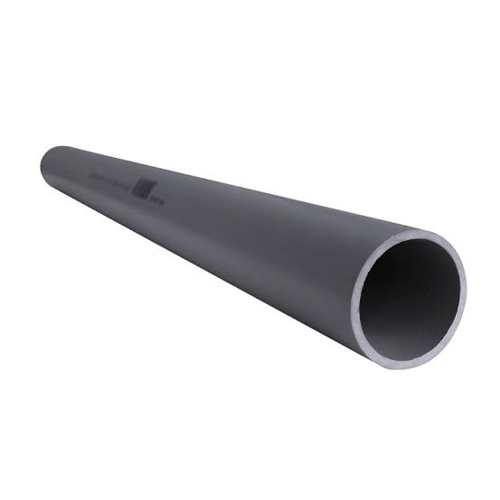
\includegraphics[height=0.5cm]{img/pvc.png} & Tour PVC de \qty{1}{m} (\qty{159}{mm} ext., \qty{144}{mm} int.) & Porte les 12 plants & 1 & \qty{1060}{XPF} & \qty{1060}{XPF} \\
\hline
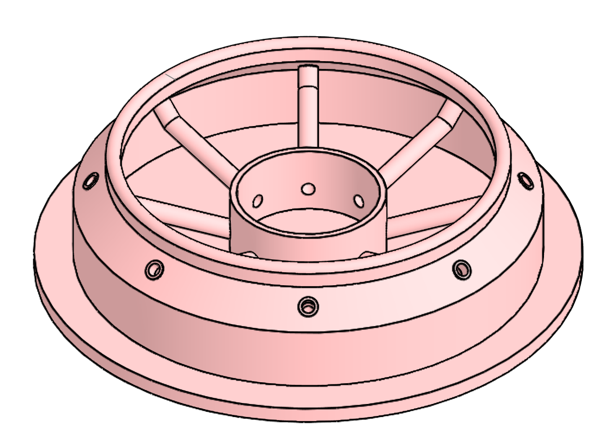
\includegraphics[height=0.5cm]{img/couvercle.png} & Couvercle répartiteur & Répartit l'eau en haut & 1 & – & – \\
\hline
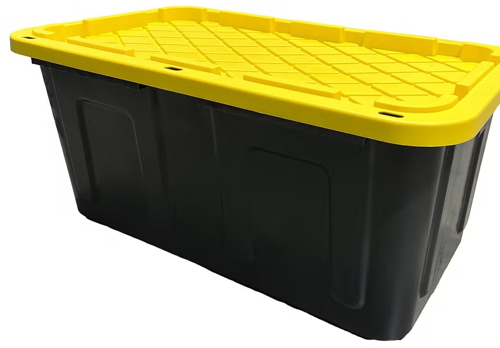
\includegraphics[height=0.5cm]{img/bac.png} & Bac de \qty{152}{L} & Réserve de solution & 1 & \qty{4160}{XPF} & \qty{4160}{XPF} \\
\hline
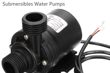
\includegraphics[height=0.5cm]{img/lpfidi.png} & Pompe de circulation \qty{12}{V} LPFIDI (Amazon) & Monte l'eau en haut & 1 & \qty{5063}{XPF} & \qty{5063}{XPF} \\
\hline
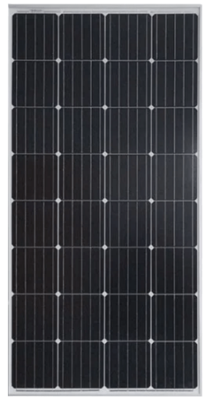
\includegraphics[height=0.5cm]{img/panneau.png} & Panneau solaire TE1250, \qty{120}{Wc} & Produit l'électricité & 1 & \qty{14320}{XPF} & \qty{14320}{XPF} \\
\hline
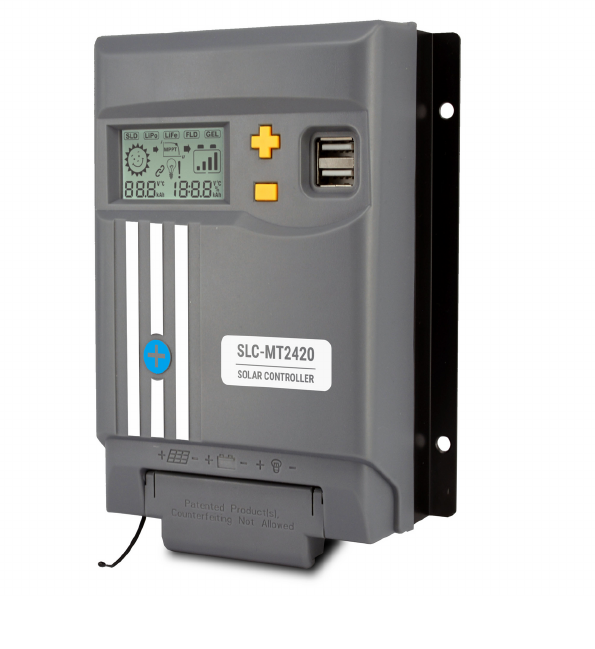
\includegraphics[height=0.5cm]{img/mppt.png} & Régulateur MPPT SLC-MT2024, \qty{20}{A} & Règle la charge & 1 & \qty{12740}{XPF} & \qty{12740}{XPF} \\
\hline
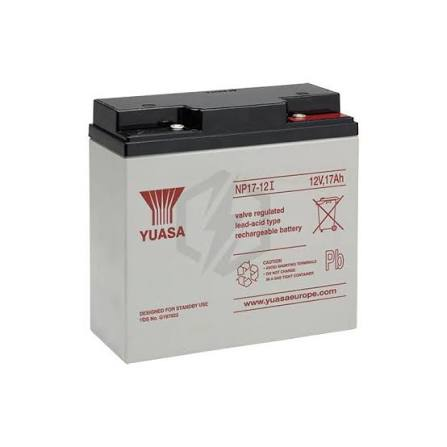
\includegraphics[height=0.5cm]{img/bat17.png} & Batterie Yuasa NP17-12I, \qty{12}{V} \qty{17}{Ah} & Stocke l'électricité & 1 & \qty{7320}{XPF} & \qty{7320}{XPF} \\
\hline
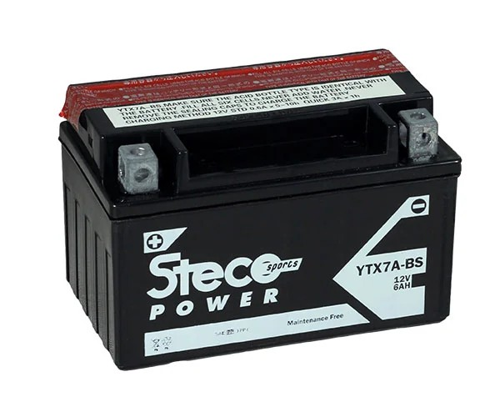
\includegraphics[height=0.5cm]{img/bat6.png} & Batterie Steco YTX7A-BS, \qty{12}{V} \qty{6}{Ah} & Stocke l'électricité & 1 & \qty{2850}{XPF} & \qty{2850}{XPF} \\
\hline
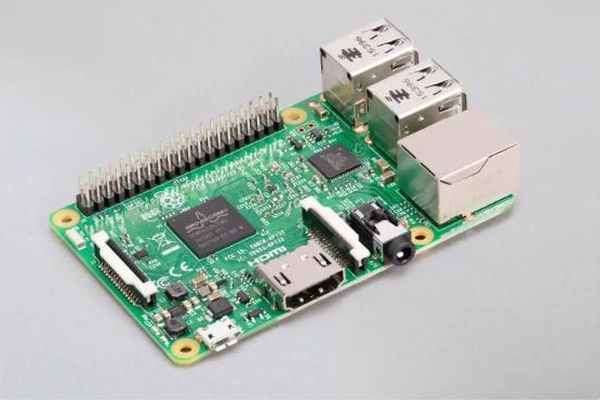
\includegraphics[height=0.5cm]{img/rpi3b.png} & Raspberry Pi 3 Model B & Le cerveau & 1 & \qty{5080}{XPF} & \qty{5080}{XPF} \\
\hline
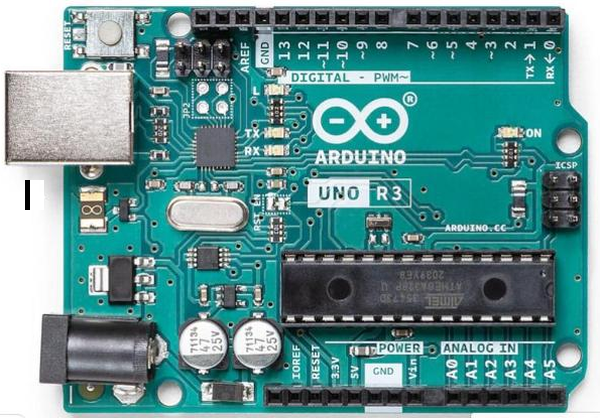
\includegraphics[height=0.5cm]{img/uno_r3.png} & Arduino Uno R3 & Exécute les ordres & 1 & \qty{2450}{XPF} & \qty{2450}{XPF} \\
\hline
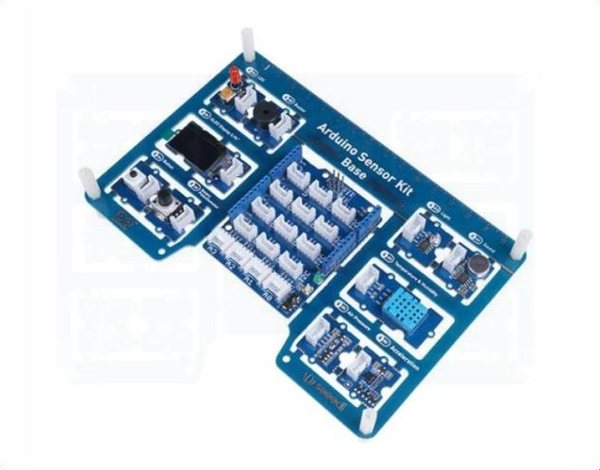
\includegraphics[height=0.5cm]{img/kit_vitta.png} & Arduino Sensor Kit (Vittascience) & Air, pression, écran, lumière & 1 & \qty{5570}{XPF} & \qty{5570}{XPF} \\
\hline
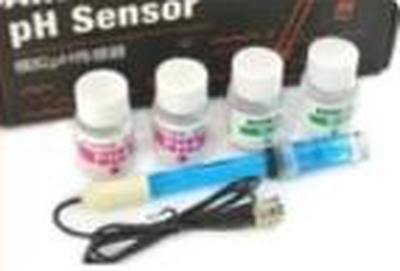
\includegraphics[height=0.5cm]{img/ph_dfrobot.png} & Sonde de pH Gravity SEN0161-V2 (DFRobot) & Mesure l'acidité & 1 & \qty{4200}{XPF} & \qty{4200}{XPF} \\
\hline
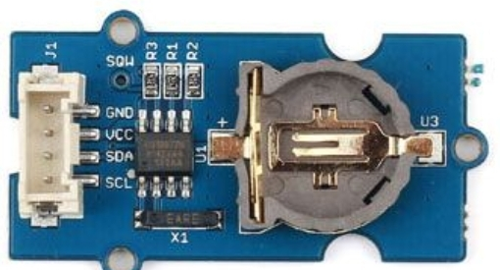
\includegraphics[height=0.5cm]{img/rtc.png} & Horloge temps réel DS1307 (Grove) & Donne l'heure & 1 & \qty{1140}{XPF} & \qty{1140}{XPF} \\
\hline
\multicolumn{6}{|c|}{\textbf{Tableau du matériel à commander pour une tour}} \\
\hline
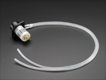
\includegraphics[height=0.5cm]{img/bom3_1.png} & Pompe péristaltique \qty{12}{V} (Adafruit) & Dosent engrais et pH & 3 & \qty{2650}{XPF} & \qty{7950}{XPF} \\
\hline
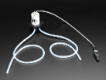
\includegraphics[height=0.5cm]{img/bom3_2.png} & Tuyau silicone d'\qty{1}{m} (Adafruit) & Tuyau de dosage & 1 & \qty{370}{XPF} & \qty{370}{XPF} \\
\hline
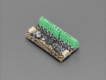
\includegraphics[height=0.5cm]{img/bom3_3.png} & Carte 8 canaux à MOSFET (Adafruit) & Commande les pompes & 1 & \qty{1590}{XPF} & \qty{1590}{XPF} \\
\hline
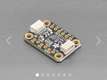
\includegraphics[height=0.5cm]{img/bom3_4.png} & Convertisseur ADS1115 (Adafruit) & Lit les sondes & 1 & \qty{1590}{XPF} & \qty{1590}{XPF} \\
\hline
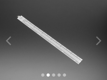
\includegraphics[height=0.5cm]{img/bom3_5.png} & Capteur de niveau eTape \qty{30}{cm} (Adafruit) & Niveau du bac & 1 & \qty{4240}{XPF} & \qty{4240}{XPF} \\
\hline
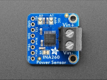
\includegraphics[height=0.5cm]{img/bom3_6.png} & Capteur INA260 (Adafruit) & Charge de la batterie & 1 & \qty{1060}{XPF} & \qty{1060}{XPF} \\
\hline
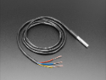
\includegraphics[height=0.5cm]{img/bom3_7.png} & Sonde de température d'eau DS18B20 (Adafruit) & Température du bac & 1 & \qty{1060}{XPF} & \qty{1060}{XPF} \\
\hline
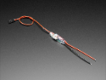
\includegraphics[height=0.5cm]{img/bom3_8.png} & Régulateur \qty{12}{V} vers \qty{5}{V} (Adafruit) & Alimente en \qty{5}{V} & 1 & \qty{1060}{XPF} & \qty{1060}{XPF} \\
\hline
\multicolumn{5}{|r|}{\textbf{Sous-total du matériel disponible}} & \textbf{\qty{65953}{XPF}} \\
\hline
\multicolumn{5}{|r|}{\textbf{Sous-total du matériel à commander}} & \textbf{\qty{18920}{XPF}} \\
\hline
\multicolumn{5}{|r|}{\textbf{Total général}} & \textbf{\qty{84873}{XPF}} \\
\hline
\end{tabularx}
\caption{Tableau du matériel de la tour : disponible et à commander.}
\end{table}

